\documentclass[a4paper,11pt]{article}
\usepackage[utf8]{inputenc}
\usepackage[T1]{fontenc}
\usepackage{amsmath, amssymb, amsfonts}
\usepackage{graphicx}
\usepackage{float}
\usepackage{booktabs}
\usepackage{geometry}
\usepackage{caption}
\usepackage{subcaption}
\usepackage{siunitx}
\usepackage{hyperref}

\geometry{margin=2.5cm}
\graphicspath{{images/}}
\title{Experimental Design for Left Ventricular Biomechanics}
\author{Diogo Amaro}
\date{\today}

\begin{document}
\maketitle

\section{Experimental Design}
\label{subsec:expdes}
To ensure thorough coverage of the input parameter space, it is important to design a framework capable of exploring every possible combination as effectively as possible. Experimental design refers to the systematic planning of physical experiments to efficiently explore a parameter space and extract meaningful insights while minimizing both number of simulations and time. Basically, a good experimental design should aim to minimize the number of runs needed to acquire as much information as possible~\cite{fang2005design}. To achieve this, various techniques have been developed and applied, four of which were initially considered and are briefly described below.


\subsection{Rectangular Grid}
Rectangular grid sampling involves discretizing each dimension of the input space into evenly spaced intervals and evaluating all possible combinations of these values across dimensions~\cite{young1991locally}. For a \( d \)-dimensional parameter space with \( n \) discretization points per dimension, the total number of sample points is given by $n^d$. Let each parameter \( q_i \in [a_i, b_i] \), for \( i = 1, \dots, d \). Then, the values for \( q_i \) are computed as
\begin{equation}
	q_i^{(j)} = a_i + \frac{j - 1}{n - 1}(b_i - a_i), \quad j = 1, \dots, n.
\end{equation}
The Cartesian product of these values across all dimensions forms the complete grid of input vectors. While straightforward, this method presents significant limitations for high-dimensional parameter spaces due to the curse of dimensionality. For a 4-dimensional parameter space, achieving reasonable resolution requires $n^4$ sample points, where $n$ represents the number of discretization points per dimension. Even modest discretization (e.g., $n = 20$) yields 160,000 required samples, making the approach computationally prohibitive for ABAQUS simulations. Because we defined our number of simulations at 10,000, the exponential scaling of computational requirements make rectangular grid sampling impractical for this study's objectives. 

\subsection{Uniform Distribution}
Uniform random sampling, also known as Monte Carlo sampling, consists of independently drawing each parameter from a uniform distribution over its domain. For each parameter \( q_i \in [a_i, b_i] \), a sample is drawn as
\begin{equation}
q_i^{(j)} \sim \mathcal{U}(a_i, b_i), \quad j = 1, \dots, N.
\end{equation}
This results in \( N \) independent samples
\begin{equation}
\mathbf{q}^{(j)} = \left( q_1^{(j)}, q_2^{(j)}, \dots, q_d^{(j)} \right)
\end{equation}
Although sampling from a uniform distribution is conceptually simple, it lacks the stratification mechanisms of more advanced sampling methods that are capable of better capturing the nonlinear relations between parameters.
\subsection{Sobol Sequence}
Sobol sequences are quasi-random low-discrepancy sequences designed to generate points that uniformly fill a multidimensional space~\cite{lemieux}. They are commonly used for numerical integration and design of experiments due to their improved space-filling properties over purely random sampling.
Mathematically, a Sobol sequence generates a sequence of points:
\begin{equation}
\mathbf{x}_i = (x_i^{(1)}, x_i^{(2)}, \dots, x_i^{(d)}), \quad i = 1, 2, \dots, N,
\end{equation}
where each component \( x_i^{(j)} \in [0, 1] \) is constructed using direction numbers and bitwise operations involving the binary representation of the index \( i \)~\cite{joe2008constructing}. The key idea is to minimize the discrepancy \( D_N \) of the point set, which quantifies how uniformly the samples cover the domain:
\begin{equation}
D_N = \sup_{B \subset [0,1]^d} \left| \frac{A(B; N)}{N} - \lambda(B) \right|,
\end{equation}
where \( A(B; N) \) is the number of sample points falling inside the axis-aligned box \( B \), and \( \lambda(B) \) is its Lebesgue measure.

Despite the theoretical plausibility, Sobol sampling is not particularly advantageous in our case, as it assumes independent and uniformly distributed dimensions, whereas the physiological parameter space considered here represents complex interactions. Moreover, if the response surface is locally nonlinear or exhibits abrupt changes, as is often the case in biomechanical systems, Sobol points may not allocate sufficient resolution to those region~\cite{burhenne2011sampling} . However, other similar studies have achieved satisfactory simulation accuracy by sampling from a Sobol sequence ~\cite{noe2019gaussian}.

\subsection{Latin Hypercube Sampling}
The Latin hypercube sampling is a stratified sampling technique, first introduced by McKay et al.~\cite{McKay}, to generate diverse and well-distributed parameter combinations across the input space of reduced material parameters $\mathbf{q} = (q_1, q_2, q_3, q_4) \in \mathbb{R}^4$.

Let the parameter space be defined as a $d$-dimensional hypercube, with each parameter \( q_i \in [a_i, b_i] \), for \( i = 1, \ldots, d \). Suppose we wish to generate \( N \) samples. In LHS, each interval \([a_i, b_i]\) is divided into \( N \) equally probable, non-overlapping intervals. Then, one value is randomly sampled from each interval without replacement. The sampled values along each dimension are then randomly paired across dimensions to form \( N \) $d$-dimensional input vectors. Formally, for each variable \( i \), define the partition:
\begin{equation}
P_{ij} = \left[ a_i + \frac{j-1}{N}(b_i - a_i),\ a_i + \frac{j}{N}(b_i - a_i) \right], \quad j = 1, \dots, N.
\end{equation}
Then, for each \( i \), randomly permute the indices \( \{1, 2, \dots, N\} \) to obtain a vector \( \pi_i \). Sample a point \( x_i^{(j)} \in P_{i,\pi_i(j)} \) uniformly, and construct the full sample:
\begin{equation}
\mathbf{q}^{(j)} = \left( x_1^{(j)}, x_2^{(j)}, \dots, x_d^{(j)} \right), \quad j = 1, \dots, N.
\end{equation}
This process ensures that each marginal distribution is uniformly sampled, while achieving better coverage of the joint space compared to pure Monte Carlo sampling. However, for designs that depend strongly on the correlation of two variables, latin hypercube sampling has little advantage over traditional Monte Carlo sampling~\cite{press1992} as much as it is guaranteed not to perform much worse. Specifically, Owen has proven that the variance of a $n_t$-point Latin hypercube sample, $\sigma^2_{LHS}$, is related to the variance of a traditional $n_t$-point Monte Carlo sample, $\sigma^2_{MC}$, by
\begin{equation}
	\sigma^2_{LHS} \leq \frac{n_t}{n_t -1}\sigma^2_{MC}, \qquad \text{where}\: n_t > 1,
	\label{eq:vlhs_vmc}  
\end{equation}
meaning that a Latin hypercube sample with $n_t$ points never leads to a variance greater than an MC sample with $n_t-1$ points~\cite{owen1997monte}.

\begin{figure}[H]
\centering
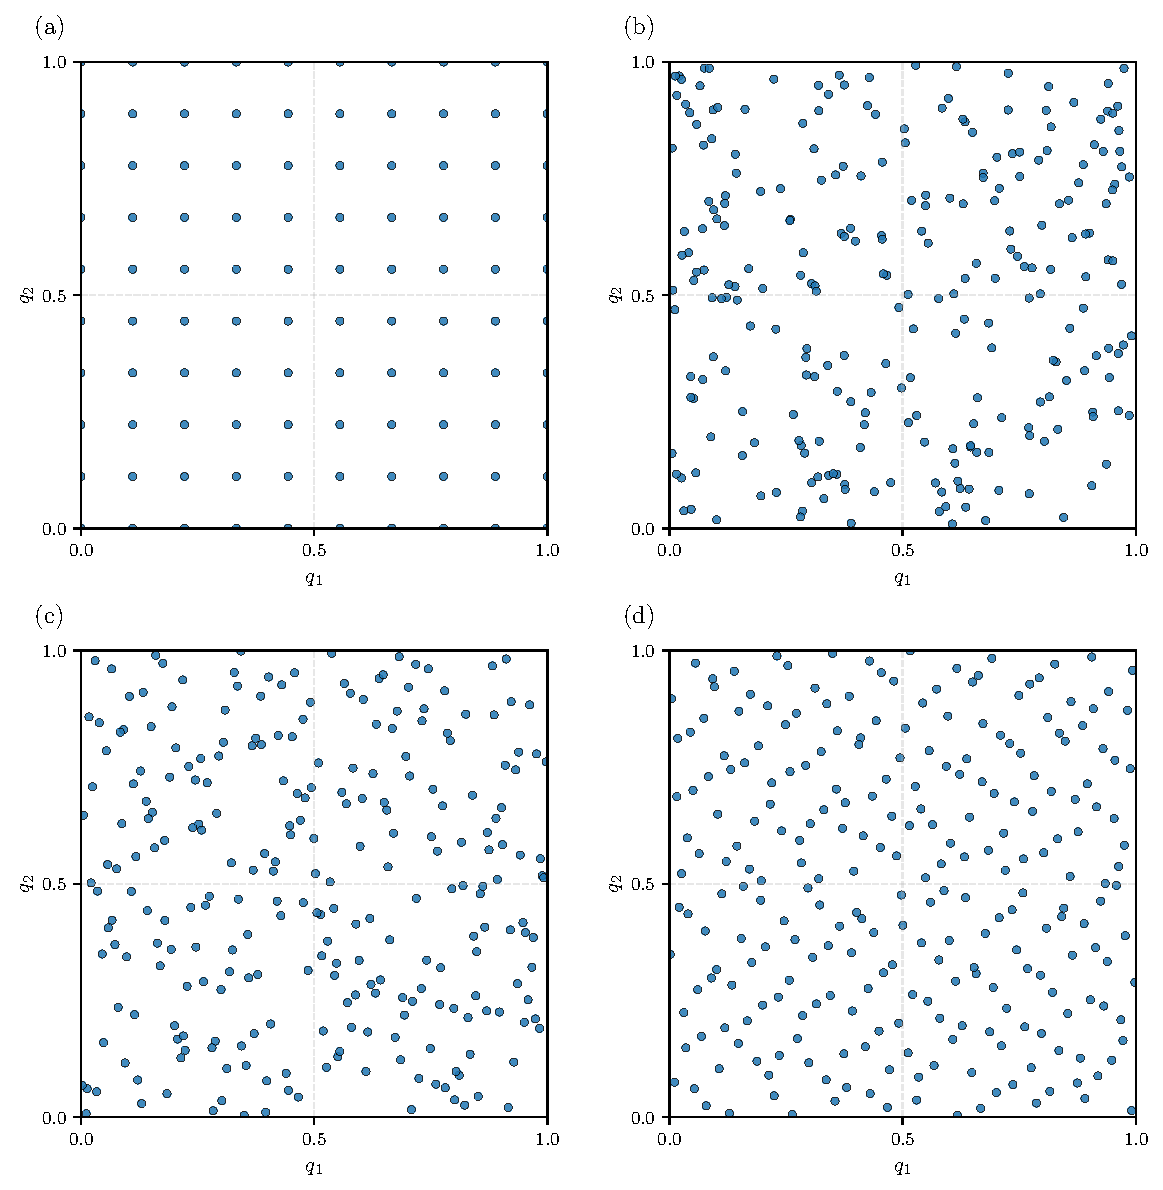
\includegraphics[width=\textwidth]{images/exp_des.pdf}
\caption{A comparison of different design choices for the training inputs. The plots show 100 points $q_i$ in the two-dimensional space \( [0,\ 1]^2 \) using different
design choices: (a) regular grid, (b) sampled from a uniform distribution, (c) Latin hypercube design and (d) from a Sobol sequence.}
\label{exp_des}
\end{figure}

Given the above considerations, the input parameter vector \( \mathbf{q} = (q_1, q_2, q_3, q_4) \) was sampled from the uniform domain \( [0.1,\ 5]^4 \) using Latin hypercube sampling with \( N = 10,\!000 \) samples. The parameter bounds were adopted from previous literature~\cite{noe2019gaussian, davies2019fast}, where they were shown to capture physiologically realistic variations in myocardial material properties. Latin hypercube sampling ensures that our surrogate models are trained on a dataset that broadly covers the entire biomechanical response space of the left ventricle. A representation of the mentioned sampling techniques is provided in Figure~\ref{exp_des}.

\bibliographystyle{ieeetr}
\bibliography{refs}

\end{document}


